\subsubsection{FIDO2}

Fast Identity Online Alliance (\acrshort{fido} Alliance) is an organisation developing authentication standards. Protocols like \acrfull{u2f}, \acrfull{uaf} or \acrshort{fido}2 are products of \acrshort{fido} Alliance and its partners.
The main aim of \acrshort{fido} is to create phishing-proof, password-less and secure standards. \acrshort{u2f} and \acrshort{uaf} have been proposed in 2014~\cite{Lindemann2014FIDOV1.0, Srinivas2014UniversalU2F}, both being updated and having new versions over time. However, new standard  \acrshort{fido}2 has been proposed, made out of two specifications: WebAuthn \cite{Balfanz2019Web1} and CTAP2 \cite{Brand2019ClientCTAP}.

The \acrshort{fido}2 project’s aim is to provide phishing-proof, password-less, secure and simple authentication protocol. Fundamental components of \acrshort{fido}2 are WebAuthn which is the \acrshort{api} for a client (by \acrshort{w3c}) and \acrshort{ctap} (by \acrshort{fido} Alliance), the \acrshort{api} for the authenticator. These define an abstraction layer which allows strongly authenticated credentials. Therefore, any supported client (a native application or a browser), running on user’s device and any supported authenticator (build-in or roaming, connected to the device via \acrshort{nfc}, \acrshort{ble} or \acrshort{usb}), can use a standardised method to authenticate the user. There are several entities involved in the process of registering and subsequently authenticating the user as it can be seen in Figure~\ref{fig:fido2_overview}.

% TODO add Caption
\begin{figure}[ht]
    \centering
    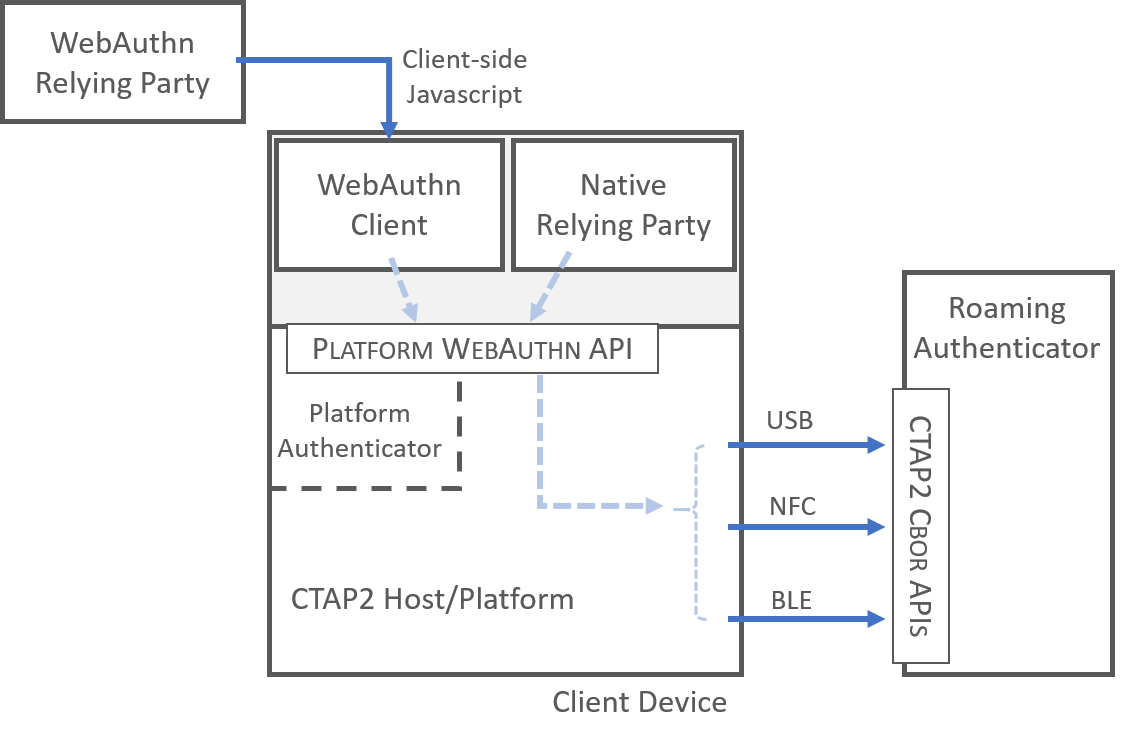
\includegraphics[width=.95\textwidth]{FIDO2_Overview}
    \caption{Explanation XYZ TODO. Taken from~\cite{Dingle2018All288910}}
    \label{fig:fido2_overview}
\end{figure}

\paragraph{Client Device} 
is a hardware which is hosting the authentication via built in or roaming authenticator and communicates with a relying party. Example of such devices are laptops or smartphones. 

\paragraph{Roaming Authenticator} 
is an authenticator which can be connected to different client devices using \acrshort{ble}, \acrshort{nfc} or \acrshort{usb} interfaces. To communicate with a client device, \acrshort{ctap}1 or \acrshort{ctap}2 can be used.

\paragraph{Platform Authenticator} 
is built in on a client device and can only be used with a given device. Example of such authenticators are fingerprint scanners or facial recognition.

\paragraph{Relaying Party} 
is an application or service which requests authenticated credentials. It can be a native or web application.

\paragraph{\acrshort{ctap}2}
\acrlong{ctap} 2 (\acrshort{ctap}2) is the newest version of the \acrshort{ctap} protocol. It is backwards compatible with the preceding \acrshort{ctap}1/\acrshort{u2f} protocol by mapping the \acrshort{ctap}2 request to the \acrshort{ctap}1/\acrshort{u2f} and vice versa for responses, unless the relaying party requests a parameter which is \acrshort{ctap}2 specific. 

The \acrshort{ctap}2 specifies the application layer protocol for communication between the authenticator and the client device, as well as how the transport layer connection with different physical authenticators should be set up in accordance with the application layer protocol. This enables external devices to be used as authenticators and work with applications and services, using WebAuthn.

The biggest improvements of \acrshort{ctap}2 over \acrshort{ctap}1 is the option to verify the user using biometrics or PIN. On top of that, besides storing a private key, devices are able to store associated metadata, which allow login even without typing a username. Android phones with Android version 7.0 and higher can also be used as authenticators, thanks to a support of Trusted Platform Modules~\cite{FIDOAlliance2019News:Key}.

\paragraph{WebAuthn} 
Web Authentication (WebAuthn) is the new web standard published in March 2019  by \acrshort{w3c}, which defines a web \acrshort{api} to enable web browsers and platforms use external authenticators via \acrshort{ctap} authentication. It standardises the public-key authentication between users and web applications or services, so it operates between the client device and a RP.

When a user wants to use authentication with \acrshort{fido}2, given application or website must support it in the first place. User can create a new account or use an already existing one and associate it with the \acrshort{fido}2 authenticator. The authenticator, whether it is a roaming or built-in one, creates cryptographic key pair (private and public key) on user request which has to be confirmed by a user gesture, e.g. fingerprint, biometrics, PIN, touch. Key pair is then created, and the private key is securely stored on the authenticator while the public key, along with associated account details is sent to the RP for storage.

In Figure~\ref{fig:fido2_authentication}, the high level sequence diagram of \acrshort{fido}2 authentication is shown. When a user wants to log-in to a service the RP sends a Credential ID and a challenge to the client, which then forwards this data to authenticator along with Relying party ID and Token binding. In order to proceed with the authentication, user's gesture is required. Relying party ID counters the man-in-the-middle attack, ensuring that it is always the same party that carries out the authentication. Credential ID allows the authenticator to have multiple accounts associated with the same key for the same service and have different key pair for each of the accounts. Authenticator then looks up the private key based on the Credential ID and Relying party ID, and uses it to sign the payload. The signed payload and a signature counter are then sent as an assertion to the client, which forwards it to the relying party together with the initial request. The relying party then verifies the signature with the public key of the given account and logs the user in. The signature counter secures the authentication from authenticator clones. In case that the authenticator is cloned and an identical authenticator is produced by a malicious party, incrementing the counter at each sign-in ensures that the state of the original authenticator and its clone divert at some point. Therefore, if the clone is used, the lower counter can be used to detect a mismatch and a possible existence of a clone.

% TODO add figure source and caption
\begin{figure}[ht]
    \centering
    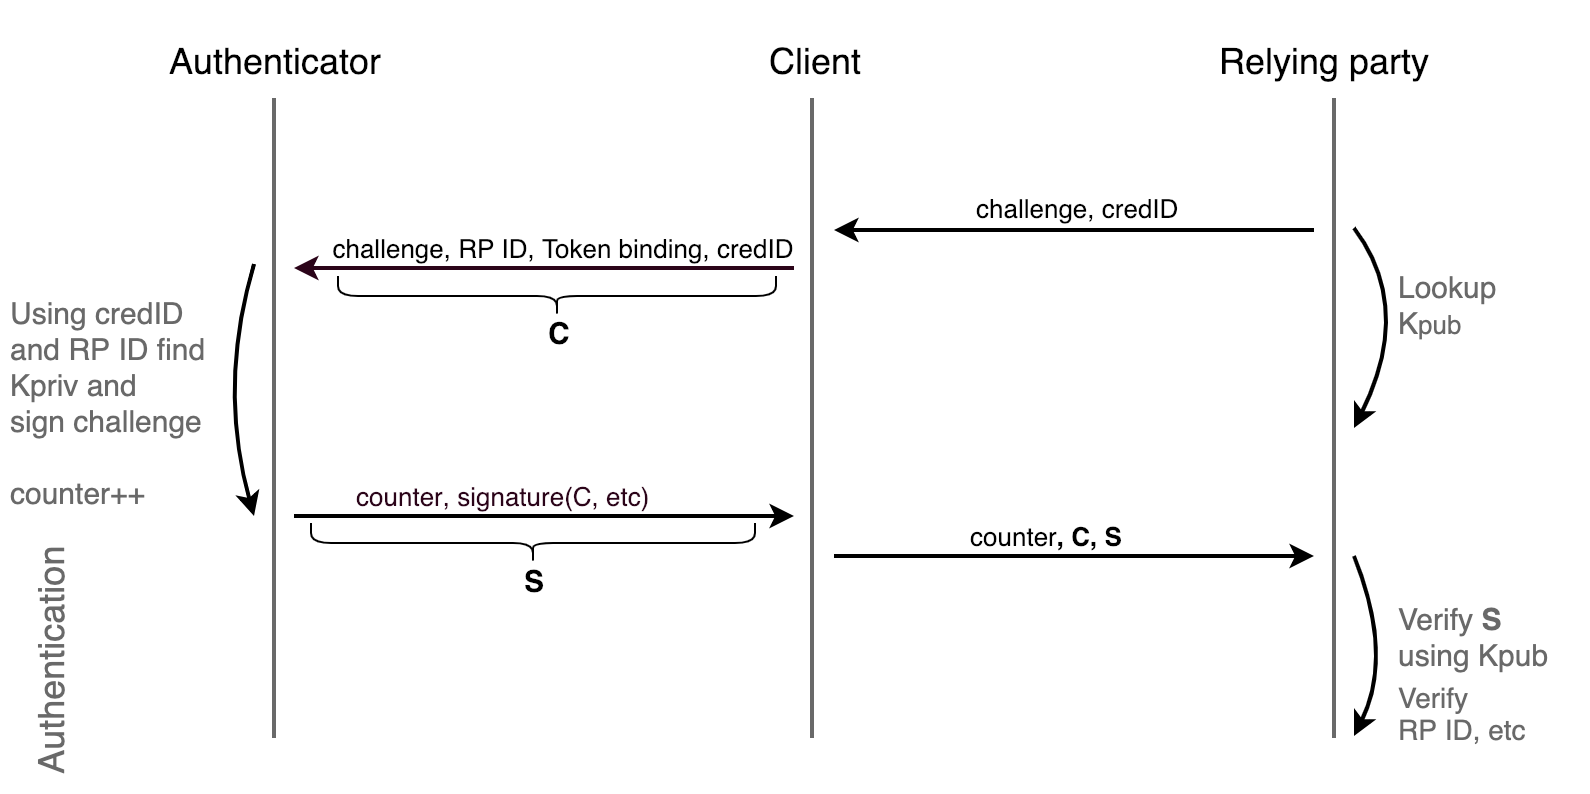
\includegraphics[width=.95\textwidth]{FIDO2_Authentication}
    \caption{Explanation. From~\cite{}SOURCE}
    \label{fig:fido2_authentication}
\end{figure}